\documentclass{report}
\usepackage[utf8]{inputenc}    
\usepackage[T1]{fontenc}
\usepackage[francais]{babel} 
\usepackage{graphicx}
\usepackage{epsfig}
\usepackage{multicol}
\usepackage{amsmath}
\usepackage{amssymb}
\usepackage{hyperref}
\usepackage[top=2cm, bottom=2cm, left=2cm, right=2cm]{geometry}
\usepackage{setspace}
\usepackage{listings}
\usepackage{color}
\usepackage[many]{tcolorbox}
\usepackage{changepage}
\usepackage{placeins}

\begin{document}

\subsection{Experimental validation of the plastic oscillator in simulation}

The simulations have been run in V-REP Simulation software with the Kinova Mico robotic arm. A gripper has been added to the robotic arm. We simulate the handshake with a ball placed inside the gripper. It moves up and down according to a 2 Hz sinusoidal signal of amplitude 0.1. Since both objects are collidable, it forces the arm to move.

The same equations mentioned previously have been used. Only the parameters were slightly changed to get better results.
The natural frequency of the oscillator depends on the values of $\tau_M$, $\tau_S$ and $\sigma_S$. Knowing that we want to be able to reach frequencies from 0 to 3.5 Hz, we chose $\tau_M = 0.35$ and $\tau_S = 3.5$ (See Figure 7). 
$\epsilon = 0.05$, $\sigma_F = 10.0$, $A_F = 0.05$ and $\tau_R = 0.005$ yield the best results for the simulation. 

\begin{figure}[h!]
\begin{center}
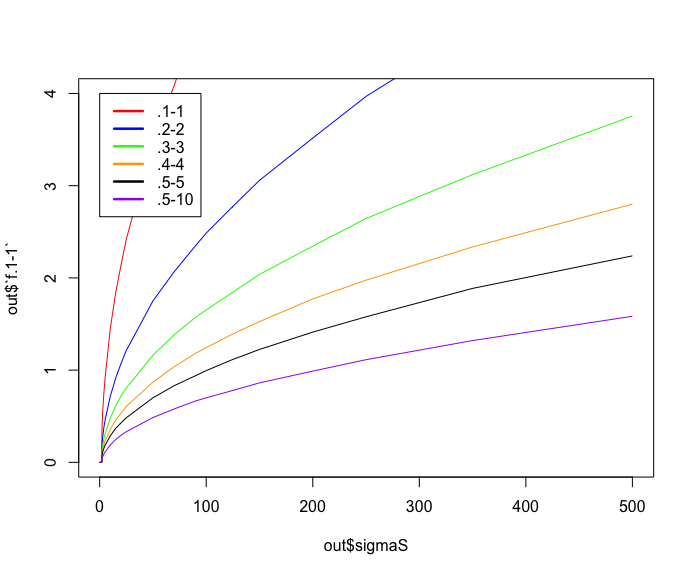
\includegraphics[width=15cm]{figures/f_ss2.png}
\end{center}
 \textbf{\refstepcounter{figure}\label{fig:05} Figure \arabic{figure}.}{Evolution of the natural frequency of the oscillator given different original values of $\sigma_S$ for various ($\tau_M$, $\tau_S$). For the handshaking process, we are interested in frequencies between 0 and 3.5 Hz. Hence, the curves suiting our purpose are (0.3, 3) and (0.4, 4).}
\end{figure}

\begin{figure}[h!]
\begin{center}
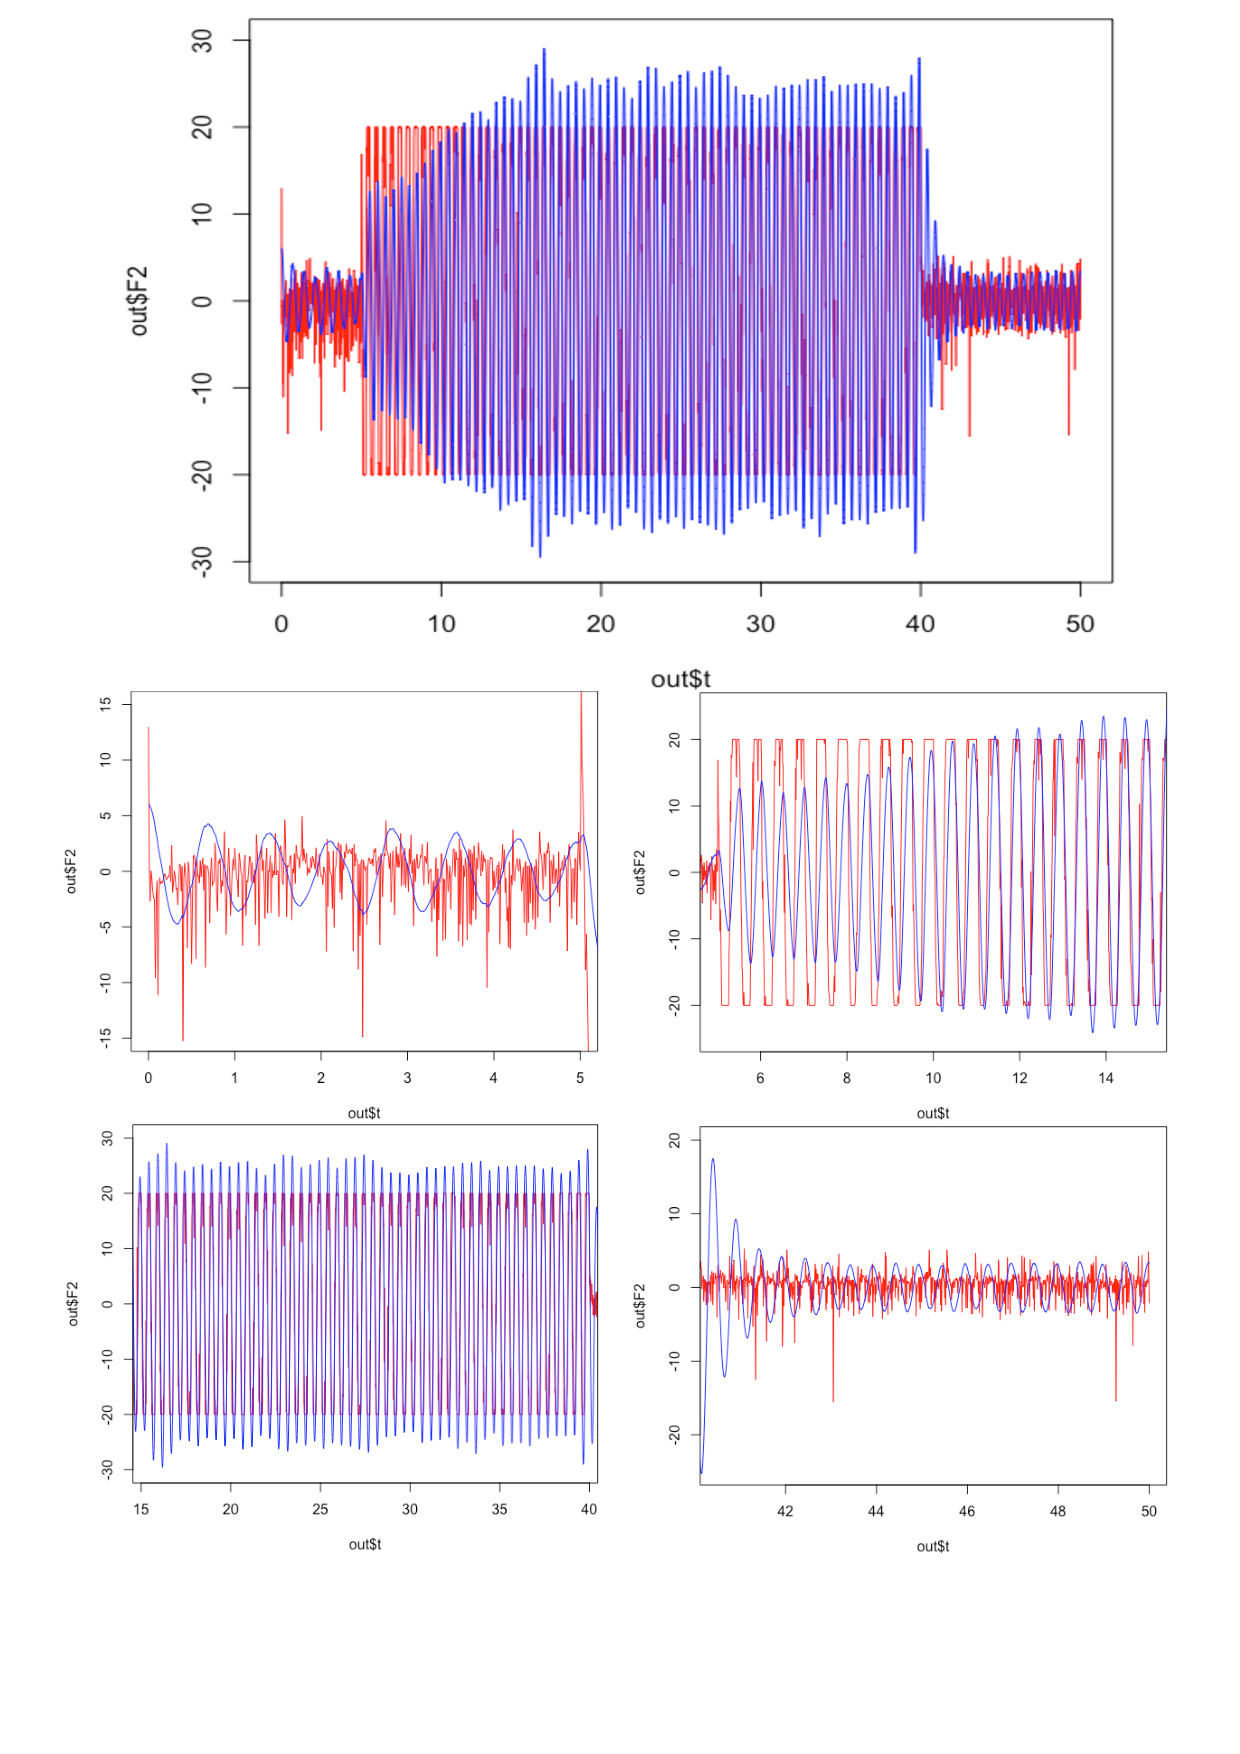
\includegraphics[width=15cm]{figures/oscillator_F2-v2.pdf}
\end{center}
 \textbf{\refstepcounter{figure}\label{fig:05} Figure \arabic{figure}.}{Evolution of V2E and F2 (Input of the cell) during the experiment. It can be divided into four parts (depicted in the bottom pictures). During the first phase, there is no physical interaction so the arm oscillates at its natural frequency. The second phase corresponds to the synchronisation phase. We can observe the natural frequency of the oscillator changing until it matches the input frequency. In the third phase, the two signals are synchronised. Finally, at 40s, the interaction stops but the arm keeps oscillating at the frequency learned during the interaction}
\end{figure}

\begin{figure}[h!]
\begin{center}
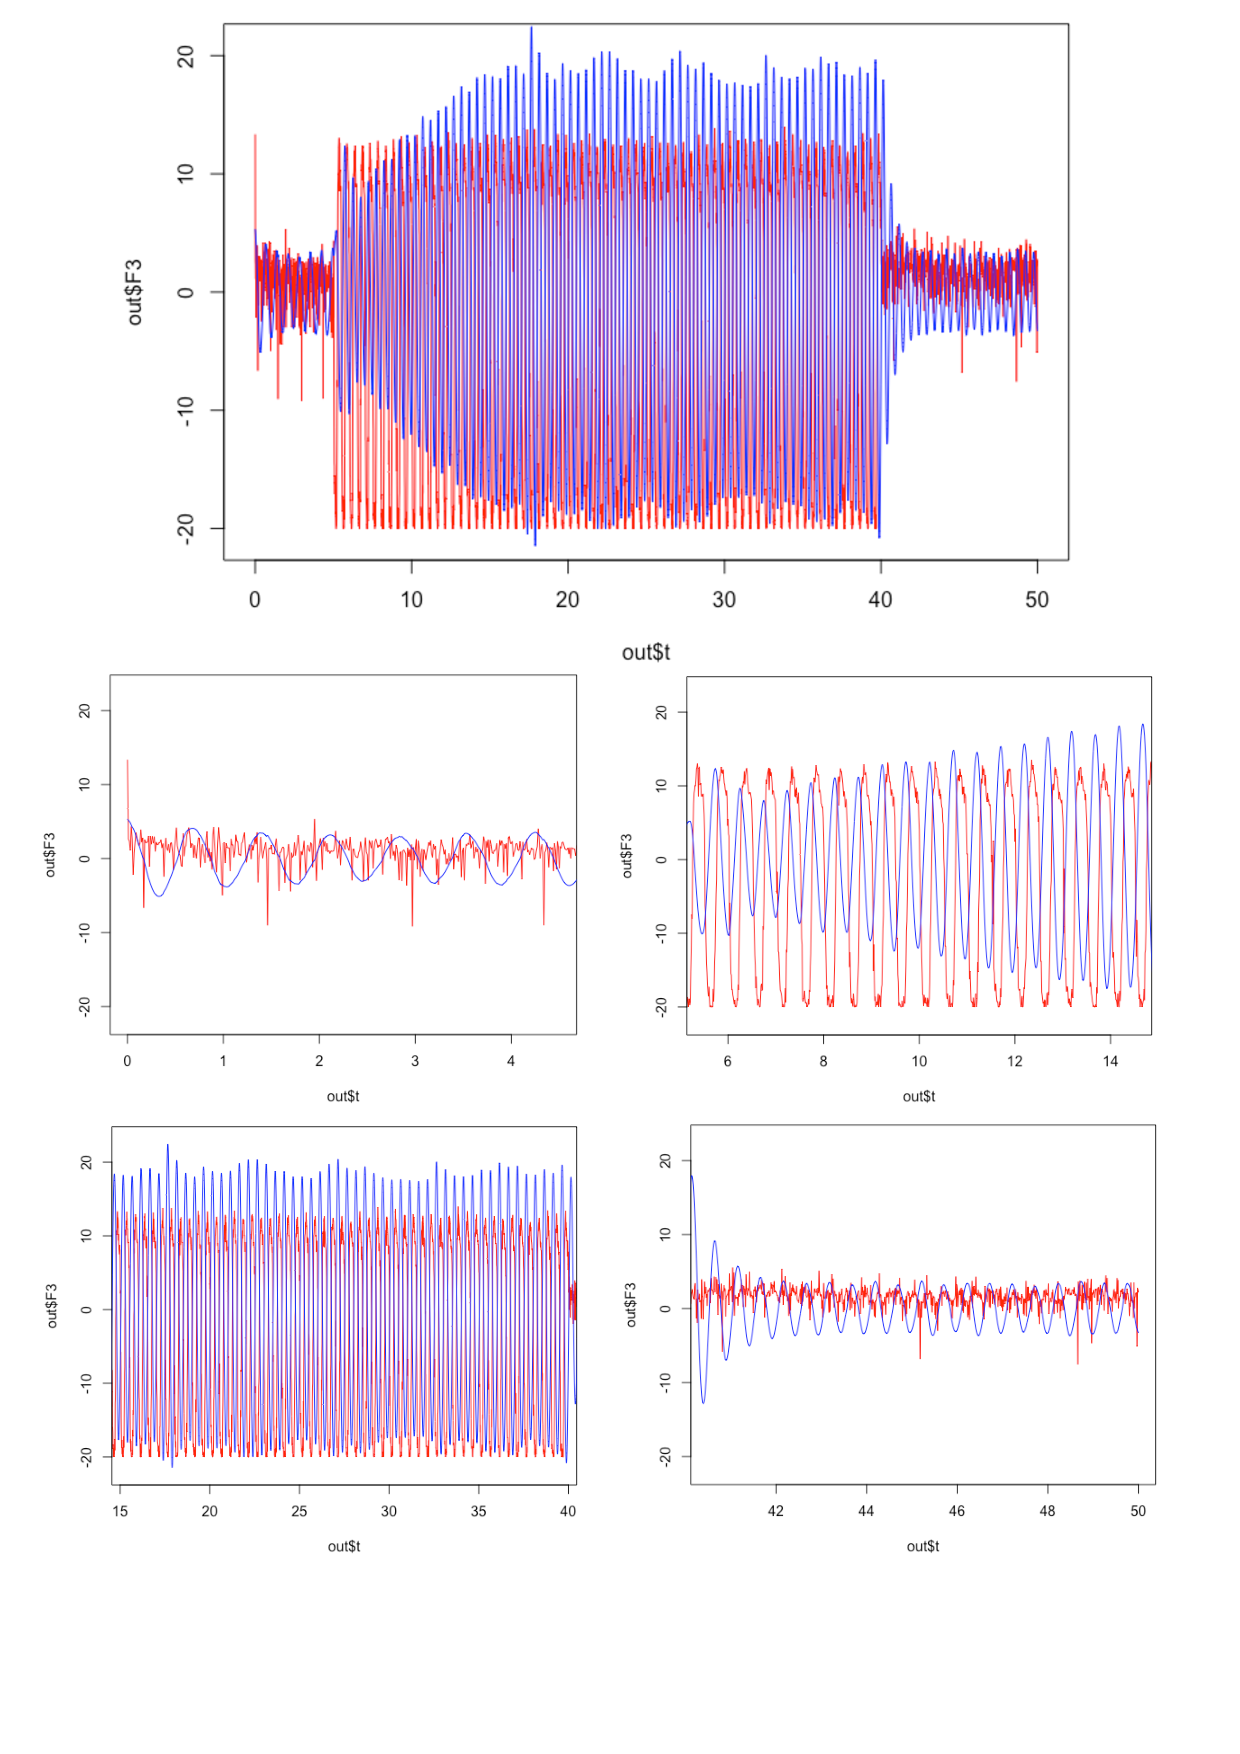
\includegraphics[width=15cm]{figures/oscillator_F3-v3.pdf}
\end{center}
 \textbf{\refstepcounter{figure}\label{fig:05} Figure \arabic{figure}.}{Evolution of V2E and F2 (Input of the cell) during the experiment. It can be divided into four parts (depicted in the bottom pictures). During the first phase, there is no physical interaction so the arm oscillates at its natural frequency. The second phase corresponds to the synchronisation phase. We can observe the natural frequency of the oscillator changing until it matches the input frequency. In the third phase, the two signals are synchronised. Finally, at 40s, the interaction stops but the arm keeps oscillating at the frequency learned during the interaction}
\end{figure}


\begin{figure}[h!]
\begin{center}
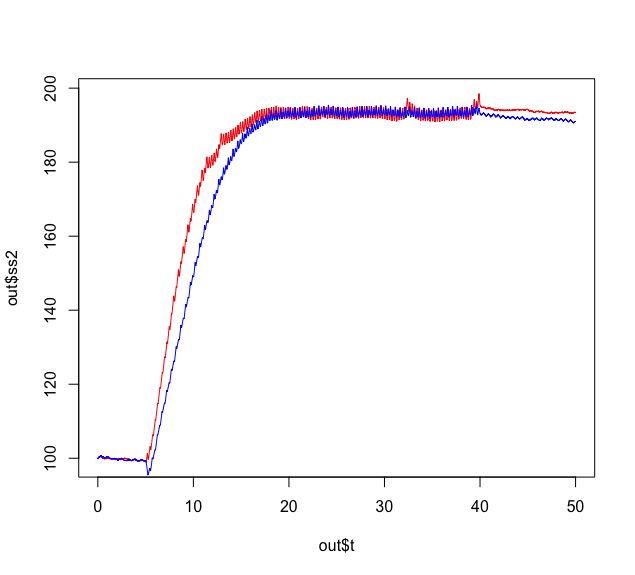
\includegraphics[width=15cm]{figures/oscillator_ss.png}
\end{center}
 \textbf{\refstepcounter{figure}\label{fig:05} Figure \arabic{figure}.}{Evolution of $\sigma_S2$ and $\sigma_S3$. The initial value is 100 for both $\sigma_S$. They stay mainly stable at 100 until t = 5 s when the interaction starts. Then they start increasing, though $ \sigma_S3$ is slightly slowler than $\sigma_S2$ but it finally catches up around t = 15 s. From t = 19 s onwards, the $\sigma_S$ are mostly stable around 190. When the interaction stops at  t = 40s, $\sigma_S$ stay stable, showing that the new value has indeed been learned.}
\end{figure}


\end{document}






